\documentclass{article}
\usepackage[utf8]{inputenc}
\usepackage[english]{babel}
\usepackage{csquotes}

\usepackage{graphicx}               % image packages
\graphicspath{ {images/} }
\usepackage{float}
\usepackage{wrapfig}
\usepackage{float,subcaption, geometry}
\usepackage[rightcaption]{sidecap}

\usepackage{pgfplots}
\pgfplotsset{compat=1.13}
\usepgfplotslibrary{statistics}

\usepackage{listings}
\usepackage{color}
\definecolor{name}{rgb}{0.5,0.5,0.5}

\definecolor{javared}{rgb}{0.6,0,0} % for strings
\definecolor{javagreen}{rgb}{0.25,0.5,0.35} % comments
\definecolor{javapurple}{rgb}{0.5,0,0.35} % keywords
\definecolor{javadocblue}{rgb}{0.25,0.35,0.75} % javadoc
\definecolor{lightgrey}{rgb}{0.9,0.9,0.9} %background colour
 
\lstset{language=Java,
frame=tb,
basicstyle=\ttfamily,
keywordstyle=\color{javapurple}\bfseries,
stringstyle=\color{javagreen},
commentstyle=\color{javagreen},
morecomment=[s][\color{javadocblue}]{/**}{*/},
numbers=left,
numberstyle=\tiny\color{black},
stepnumber=1,
numbersep=10pt,
tabsize=4,
showspaces=false,
showstringspaces=false,
breaklines=true}

\usepackage[
backend=biber,
style=alphabetic,
citestyle=authoryear-comp 
]{biblatex}
 
\addbibresource{cs4203_bib.bib}     %imports bib file

\usepackage{hyperref}
\hypersetup{
    colorlinks,
    citecolor=black,
    filecolor=black,
    linkcolor=black,
    urlcolor=black
}

\title{CS4203 Computer Security Practical 2: \\ Rhythmic Keylogger for Authentication}
\author{120011995}
\date{Due Date: 7 March 2016}

\begin{document}

\maketitle

\section{Introduction}
\paragraph{}
A keylogger is a computer program developed for the purpose of monitoring and tracking what keys are entered on a computer keyboard. Whether this is a traditional desktop/laptop computer or a virtual mobile phone keyboard is irrelevant the program seeks to identify the keys that have been pressed. There are numerous legitimate use cases for keylogging, such as, auditing and accountability of computer usage in an office environment, as well as monitoring a person's mobile phone usage to ensure they do not incur any additional charges. However these programs can also be utilised to compromise the security of a system by collecting login credentials via monitoring of inputs. Passwords are not a truly unique identification mechanism, as if an attacker gains access to a valid pairing of username and password they an easily enter these into the system and gain access to sensitive information. Thus, there has been much research conducted to identify new methods of authentication such as, Passfaces \parencite{Dunphy}, Draw-a-Secret (DAS) \parencite{DunphyYan}, Background
Draw-a-Secret (BDAS) \parencite{DunphyYan}. Although many of these processes work effectively, they suffer from new limitations such as memory decay which limits their practicality as a silver bullet to the problem of authentication. This has prompted researchers to identify areas which uniquely identify users and a hypothesis is that a password coupled with the rhythm and cadence at which a user types is more secure than the password on its own. This paper will explore this hypothesis and provide experimental evidence on the viability of using a rhythmic keylogger in conjunction with a password to improve the security of authentication.         

\section{Problem Statement}
\paragraph{}
Users spend a large proportion of time using computer systems typing inputs via a keyboard. Therefore users develop an individual technique of typing and implement  largely unique patterns when typing. The view of current research is that a profile of the patterns used in typing could be utilised to authenticate users together with a valid username and password combination. 

\paragraph{}
The typing pattern on a keyboard is considered a biometric behavioural characteristic that can be used to identify or authenticate users, the study of this discipline is called keystroke dynamics \parencite{keyStrokeDynamics}. The field of keystroke dynamics focuses on two differing areas of analysis, ``fixed text" and ``free text". Fixed text enforces that all users type the same sample of text, such as username and password combination or a small phrase. In contrast to this free text allows for all inputs by a user to be inspected, which is a much more powerful application of key stroke dynamics, allowing it to be applied to a larger number of applications. However, this comes at the expense of an increase in complexity of experimentation and computation as the free text does not have fixed, easily extracted characteristics \parencite{sznur2015advances}. The experiment conducted for this practical utilises the paradigm of fixed text, to ensure a measurable comparison of the rhythm used by users to type a set phrase. 

\section{Relevant Background} \label{background}
% History use of morse code 
\paragraph{}
The monitoring of human characteristics for identification purposes during interaction with machines has been prevalent since morse code communication in World War 2. As each operator had their own unique typing style, closely listening to the typing rhythm of an operator could be used to effectively identify them \parencite{sznur2015advances}. The techniques utilised in this process have been extended upon to create the current keystroke dynamics algorithms. 

\paragraph{}
% Research attempts at cadence monitoring Cite some papers and their attempts
Early research in the field of fixed text keystroke dynamics looked to improve the accuracy of the approach to ensure its viability in practice \parencite{Bergadano:2002}. To facilitate easier testing of fixed text keystroke dynamics systems, researchers complied a dataset of the typing rhythm data
of volunteer users to enable rapid testing of systems \parencite{bello2010collection}. There has been much more success in development of fixed text systems as the complexity of algorithms and reliance on computing resources is vastly reduced in comparison to free text implementations. 

\paragraph{}
Much research has been conducted in the area of keystroke dynamics for free text, early work of \parencite{Gunetti:2005}, presented a method to compare typing samples of free text that could used to verify personal identity. The authors of this paper  presented the foundations of the idea of ``continuous authentication", which is the ability of a system  to constantly verify if the current user is the one who originally logged in \parencite{sznur2015advances}. Furthermore, they argued the premise stated earlier in this report that keystroke dynamics can be useful in computer security as a complementary or alternative method to user authentication and as an aid to intrusion detection \parencite{Gunetti:2005}. The ideas proposed in this early paper have been developed upon by numerous research such as \parencite{contFreeText} and \parencite{sznur2015advances} which both look to further improve the paradigm of continuous authentication. 

\paragraph{}
% Keystroke Dynam Authentication
Keystroke dynamics has proved to form a robust defence, improving the security of authorisation as there has yet to be a successful attack on a solidly built keystroke dynamics system \parencite{sznur2015advances}. This is in stark contrast to a system simply secured by passwords, as human nature dictates that users will use simple passwords to ensure they remember them. This is combination with the range of attacks that can be utilised to obtain a password such as social engineering, spyware, dictionary attack and mere brute force attacks \parencite{alsultan2013keystroke}. A keystroke dynamics system makes all of these approaches redundant. Systems simply secured by the username password techniques suffers from the security-usability trade-off dilemma \parencite{alsultan2013keystroke}, as they look to offer usability at the expense of security. Numerous other authentication techniques have been suggested however if they sacrifice usability for security they are unlikely to be widely adopted due to user pressure. This is why keystroke dynamics is an effective solution to the authentication problem, as it requires no further memory or interactions from the user, simply their typing behaviour which is used regardless when typing in authentication credentials, yet it provides a dramatic increase in security. The technique has not been perfected but it is an active research area which looks to improve the complexity and reliability of the techniques utilised to identify a user by their typing characteristics \parencite{sznur2015advances}. 

\paragraph{}

The future of keystroke dynamics research will most likely surround the ideal of continuous authentication which improves upon the simplistic approach keystroke dynamics only upon entry to a system. In addition, implementations of keystroke dynamics systems are available on a variety of devices available today, an effective solution has created for mobile phones \parencite{maiorana2011keystroke} which has the potential to generalise to a large proportion of mobile devices.  

\paragraph{}
% Current industry attempts at cadence monitoring 
There have also been copious attempts to utilise keystroke dynamics in industry. For example, Scout Analytics developed technology for its clients to stop people sharing user accounts without permission, i.e. giving a friend or colleague the id and password to their account so they can access the features of a paying subscriber. This looked to stop organisations buying a single account for an expensive resource and sharing this across an entire office. Scout used some Javascript timing features to watch how users type when they enter their login credentials for various services. The algorithms implemented need a minimum of 5 attempts at entering a phrase with a length of 12 characters in order to generate a typing ``cadence" \parencite{arsTech}. By utilising repeated logins the system could analyse the cadences and place them into distinct categories of digital patterns, each of which was assigned a digital serial number, which is utilised to ensure multiple different users are not logged on at once. A limitation of this approach is that the typing patterns are not globally unique, Scout suggests that 1 in 20,000 people share the same pattern, although the pattern can be combined with IP addresses and browser information, to uniquely identify a user for Scout's purposes \parencite{arsTech}. 

\section{Experiment Design and Setup} \label{experiment}
\paragraph{}
The framework used for this experiment was a Java program, important areas of the program can be found in Appendix Section \ref{appendix}. A high level description of its functionality can be seen below in Section \ref{setup}. 

\subsection{Experiment Framework} \label{setup}
\paragraph{}
For this practical I created a Java program which utilises the Java Interface KeyListener to monitor the keyboard input of the user and compile a typing timings profile per user. Along with this monitoring I implemented a simple Java Swing User Interface (UI) to facilitate registration and login of users. The program keeps persistent storage of User objects by serialising them and writing them to a file, which can be subsequently read and the objects re-created whenever the program is launched. This process utilises the Java Serializable API which allows objects to be stored as a file. To facilitate easy and as repeatable as possible experimentation I implemented the Logger class which was used to output the results of the experiment to a text file which could then be analysed and statistically reported upon. Another notable design feature was implementing a class for User objects so that they could be easily manipulated and stored throughout the entire program. Along with this as this practical was in the context of a Computer Security module I used the SHA-256 cryptographic one-way hash function to encode the passwords of users, thus ensuring the secure storage of user's passwords.       
\paragraph{}
Figure \ref{fig:register} shows an example of a form used to gain a profile of the user's typing rhythm  whilst they enter login credentials, this form is for password only another form was created when ID and Password were monitored. The UI is very simplistic but as this was not part of the requirements I did not want to spend time improving this as it had no impact on the functionality of the program or the success of the experiment. 

\begin{figure}[H]
    \centering
    \includegraphics[width=0.2\textwidth]{register}
    \caption{User registration form}
    \label{fig:register}
\end{figure}

\paragraph{}
Figure \ref{fig:id_same_val} to Figure \ref{fig:timings_pass} shows the UI response when a user inputs incorrect details during the registration phase. This can be caused by entering either null or empty strings in the username or password input fields or by not typing the same password correctly in each password input field. 

\begin{figure}[H]
    \centering
    \includegraphics[width=0.6\textwidth]{id_same_val}
    \caption{When a user inputs username values which do not match}
    \label{fig:id_same_val}
\end{figure}

\begin{figure}[H]
    \centering
    \includegraphics[width=0.6\textwidth]{timings_id}
    \caption{When the timing profiles for the entry to the username fields do not match}
    \label{fig:timings_id}
\end{figure}

\begin{figure}[H]
    \centering
    \includegraphics[width=0.6\textwidth]{pass_vals}
    \caption{When a user inputs password values which do not match}
    \label{fig:pass_vals}
\end{figure}

\begin{figure}[H]
    \centering
    \includegraphics[width=0.6\textwidth]{timings_pass}
    \caption{When the timing profiles for the entry to the password fields do not match}
    \label{fig:timings_pass}
\end{figure}

Once a user has successfully registered they can then return to the Login form and input their details. Figure \ref{fig:login} shows the Login screen of the UI. 

\begin{figure}[H]
    \centering
    \includegraphics[width=0.3\textwidth]{login}
    \caption{User login form}
    \label{fig:login}
\end{figure}

\paragraph{}
Along with checking the username and password of a user, the program will compare the typing rhythm of the user to  the profile set during registration. If the users credentials do not match some stored by the program or their typing characteristics are different than the profile set during registration the login attempt with be rejected. Figure \ref{fig:wrong_creds} shows the output when the user enters incorrect credentials whilst Figure \ref{fig:typing_cadence} shows an unsuccessful login attempt due to incorrect typing characteristics.


\begin{figure}[H]
    \centering
    \includegraphics[width=0.4\textwidth]{wrong_creds}
    \caption{When a user inputs incorrect credentials i.e. no match can be found in stored users}
    \label{fig:wrong_creds}
\end{figure}

\begin{figure}[H]
    \centering
    \includegraphics[width=0.4\textwidth]{typing_cadence}
    \caption{When a user's typing characteristics do not matched those stored}
    \label{fig:typing_cadence}
\end{figure}

This can be contrasted to Figure \ref{fig:successful_login} which shows a user who has successfully logged on and receives a congratulations message along with their user ID.

\begin{figure}[H]
    \centering
    \includegraphics[width=0.4\textwidth]{successful_login}
    \caption{Successful Login displaying the user's ID and a congratulations message}
    \label{fig:successful_login}
\end{figure}

\subsection{Experiment Design}
\paragraph{}
The overall objective of this experiment was to explore the hypothesis that a password coupled with the normal rhythmic typing of the owner is more secure than the password on its own. The experiment will essentially assess the viability of adding the typing characteristics of an owner into the traditional username and password credentials authentication. 

\paragraph{}
For the purpose of this experiment a pattern is defined as ``a mix of rhythms with perhaps more than 2 complicated timings mixed together or one with fixed or relational times between each keystroke. A simple pattern is the same rhythm as in ta-ta-ta-ta but a patterned example could be a user thinking of a song or a marching or clapping rhythm and keying the strokes according to that melody". 

\paragraph{}
I chose to gain a profile of the user by requesting them to type their username twice and password five times. This would allow me to ensure the rhythmic performance of the user was consistent across a multitude of results and was not an outlying result. I utilised 10 participants to test each of the hypotheses and each participant entered their credentials 10 times for each hypothesis. I would to thank the participants and acknowledge them for their time.

\paragraph{}
All experiments were conducted with a tolerance of 100ms (0.1 of a second) between the timing values within each login attempt and the stored typing profile values. 

\paragraph{}
For most of the hypothesis presented I conducted a paired sampled (within subjects) t test to measure whether the results of the two conditions of the experiments were statistically different from one another. I therefore set up each experiment to contain a null hypothesis H0 which assumes there is no significant difference  between the two result sets. The experiment would also contain H1 which assumes that there is a significant difference between the two sets of results. For all experiments in this practical I used the significance level of 5\% (0.05) as this is a widely accepted research standard. Therefore, if the calculated p value of the t-test was less than 0.05 then the difference is significant therefore we can reject the null hypothesis, otherwise if the p value is greater than 0.05 then the results show that the difference is not significant and we fail to reject the null hypothesis. All statistics calculated for this report can be found in the \textit{Statistics} spreadsheet file in the project directory. The t test approach was not suitable to be applied to hypothesis 4 as I had included 3 values therefore this uses the formulae suggested in the specification.  \\

\section{Experiment Results}

\subsection{Hypothesis 1}
\begin{center}
\textit{Compare	(expected) rhythms	from	repeated	keys	or	pairs	of	keys against	passwords that are	distributed	around	the	keyboard.} \newline \\

\textbf{H0:} \textit{There	is	no significant	difference	in	the	success	(or	failure)	rate	of	simple	vs	complex	(distributed)	rhythms,	that	is	neither has	a	radically	higher	or	lower	access	or	denial	rate	than	the	other.} \newline \\

% There is a diff and it those that are simple in one area are more successful than those distriubted
\textbf{H1:} \textit{There is a difference in the	success	(or	failure)	rate	between	simple password rhythms	and	more complex rhythms.}
\end{center}

To test the first hypothesis I assigned each participant with an ID and Password pairing which contained a simple rhythm of repeated pairs of keys: ID: aaaaaa and Password: a1a1a1. I then assigned each of the participants a pairing of more distributed credentials: ID: b0a9e8 and Password: zpxjc6. This pairing involved keys that were more distributed around the keyboard and contained a slightly more complex pattern. I then asked each participant to register their ID and password combination and then attempt to login. The results of the user trial with both the simple repeated keys pattern and the complex distributed rhythm passwords is shown in Table \ref{table:1}. 

{
\begin{table} [H]
\centering
% TODO Table: First 5 participants simple rythm password
\begin{tabular}{ |p{2cm}|p{4cm}|p{4cm}| p{4cm} | }
\hline
\multicolumn{4}{|c|}{\textbf{Hypothesis 1 Testing Results}} \\
\hline
\textbf{Participant} & \textbf{Success Repeated Keys} & \textbf{Success Distributed Keys} & \textbf{Total Success Percentage} \\
\hline
1 & 8 & 6 & 70\% \\
\hline
2 & 7 & 5 & 60\% \\
\hline
3 & 8 & 6 & 70\% \\
\hline
4 & 7 & 7 & 70\%  \\
\hline
5 & 6 & 4 & 50\% \\
\hline
6 & 5 & 6 & 55\% \\
\hline
7 & 6 & 7 & 65\% \\
\hline
8 & 5 & 5 & 50\% \\
\hline
9 & 9 & 7 & 80\% \\
\hline
10 & 7 & 7 & 70\% \\
\hline
\textbf{Total} & \textbf{68} & \textbf{60} & \\
\hline
\textbf{Average} & \textbf{6.8} & \textbf{6} & \textbf{64\%} \\
\hline
\textbf{Maximum} & \textbf{9} & \textbf{7} & \textbf{80\%} \\
\hline
\textbf{Minimum} & \textbf{5} & \textbf{4} & \textbf{50\%} \\
\hline
\textbf{Range} & \textbf{4} & \textbf{3} & \textbf{30\%} \\
\hline
\textbf{Median} & \textbf{7} & \textbf{6} & \\
\hline
\textbf{Lower Quartile} & \textbf{6} & \textbf{5.25} & \\
\hline
\textbf{Upper Quartile} & \textbf{7.75} & \textbf{7} & \\
\hline
\end{tabular}
\caption{Table shows results of testing for hypothesis 1}
\label{table:1}
\end{table}
}

As shown in the table the total number of successes for the simple repeated keys pattern was 68 and the total successes with a more distributed pattern was 60. The average number for the participants entering a simple pattern was 6.8 whilst this decreased to 6 when a distributed password was introduced. Further highlighting this trend of more successes using repeated keys was the median value which was 7 for the repeated keys pattern and 6 for the complex distributed patterned password. Overall it is evident from the table that users had more success logging in when given a simple repeated keys pattern in comparison to a password which contained a pattern of keys distributed around the keyboard. The results of this experiment are graphically presented as a box plot in Figure \ref{fig:boxPlotHyp1}, which shows that the results are similar to one another, as they largely overlap.    

\begin{figure} [H]
    \centering
    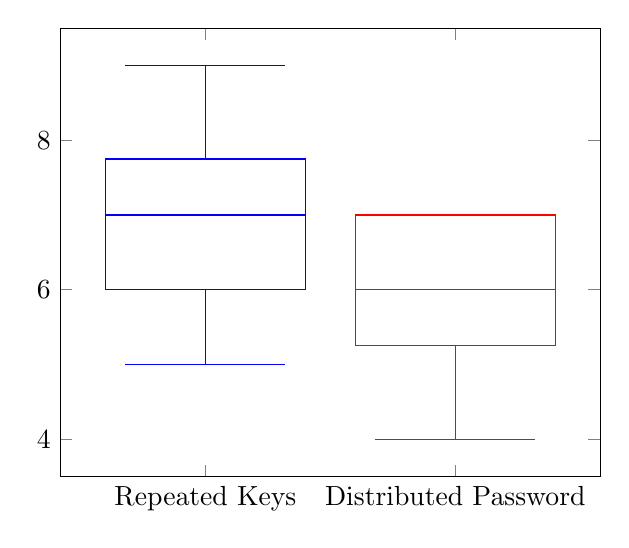
\begin{tikzpicture}
  \begin{axis}
    [
    boxplot/draw direction=y,
    xtick={1,2},
    xticklabels={Repeated Keys, Distributed Password},
    ]
    \addplot+[
    boxplot prepared={
      median=7,
      upper quartile=7.75,
      lower quartile=6,
      upper whisker=9,
      lower whisker=5
    },
    ] coordinates {};
    \addplot+[
    boxplot prepared={
      median=6,
      upper quartile=7,
      lower quartile=5.25,
      upper whisker=7,
      lower whisker=4
    },
    ] coordinates {};
  \end{axis}
\end{tikzpicture}
    \caption{The results of Hypothesis 1 Testing.}
    \label{fig:boxPlotHyp1}
\end{figure}

The results of the t test for this returned the value 0.043421145 which is $<$ than 0.05, therefore the difference is statistically significant. Thus, we can reject the null hypothesis and accept H1 which states there is a difference in the	success	(or	failure) rate between simple password rhythms and	more complex rhythms. These results show that users were more successful when logging in with a simple pattern of keys which were located near one another in comparison to a distributed pattern of keys. The resulting p value is however close to the threshold value therefore this experiment may require further research to ensure this value is consistent. 

\subsection{Hypothesis 2}
\begin{center}
\textit{That some patterns are more easily detected or broken than others.} \newline \\

% H0 for this one as there is no sig difference between different patterns
\textbf{H0:} \textit{That	there	is no significant difference in	the	detection (access)	rate	between	a	simple	and	a	complex	pattern	of	a password.} \newline \\
\textbf{H1:} \textit{That	there	is a significant difference in	the	detection (access)	rate	between	a	simple	and	a	complex	pattern	of	a password.} \newline \\
\end{center}

To test the hypothesis for this section I assigned the users the following ID and Password for the simple pattern, ID: aaaaaa, Password: a1a1a1. I then assigned the users a more complex ID and Password pairing of ID: qwebnm, Password: a2b3c4. The second password contains a much more complex pattern which will facilitate a comparison between simple and complex patterns within the passwords. 

{
\begin{table} [H]
\centering
% TODO Table: First 5 participants simple rythm password
\begin{tabular}{ |p{2cm}|p{4cm}|p{4cm}| p{4cm} | }
\hline
\multicolumn{4}{|c|}{\textbf{Hypothesis 2 Testing Results}} \\
\hline
\textbf{Participant} & \textbf{Success with Simple Pattern} & \textbf{Success with Complex Pattern} & \textbf{Total Success Percentage} \\
\hline
1 & 7 & 6 & 65\% \\
\hline
2 & 8 & 7 & 75\% \\
\hline
3 & 7 & 4 & 55\% \\
\hline
4 & 6 & 6 & 70\%  \\
\hline
5 & 6 & 4 & 50\% \\
\hline
6 & 5 & 6 & 55\% \\
\hline
7 & 8 & 7 & 75\% \\
\hline
8 & 6 & 4 & 50\% \\
\hline
9 & 7 & 7 & 70\% \\
\hline
10 & 6 & 5 & 55\% \\
\hline
\textbf{Total} & \textbf{66} & \textbf{56} & \\
\hline
\textbf{Average} & \textbf{6.6} & \textbf{5.6} & \textbf{61\%} \\
\hline
\textbf{Maximum} & \textbf{8} & \textbf{7} & \textbf{75\%} \\
\hline
\textbf{Minimum} & \textbf{5} & \textbf{4} & \textbf{50\%} \\
\hline
\textbf{Range} & \textbf{3} & \textbf{3} & \textbf{50\%} \\
\hline
\textbf{Median} & \textbf{6.5} & \textbf{6} & \\
\hline
\textbf{Lower Quartile} & \textbf{6} & \textbf{4.25} & \\
\hline
\textbf{Upper Quartile} & \textbf{7} & \textbf{6.75} & \\
\hline
\end{tabular}
\caption{Table shows results of testing for hypothesis 2}
\label{table:2}
\end{table}
}

As shown by Table \ref{table:2} the total number of successful logins using a simple pattern password was 66 whilst this decreased to 56 when a complex pattern was utilised. The average also shows that simple patterns granted more successful logins as it was 6.6 which again fell to 5.6 when a complex pattern was utilised. The median values also affirm the idea that simple passwords allow for more successful logins as the median for simple passwords was 6.5, in contrast the median of complex patterned passwords was 6. Overall the table shows that users had an easier time authenticating with a simple pattern as opposed to a complex pattern. The results of this table are illustrated in Figure \ref{fig:boxPlotHyp2}, which shows the results for a simple pattern were much less sporadic largely concentrated between 6 and 7, whilst the success of the complex ranged from 4.5 to 6.5. There also a small overlap between the plots.  

\begin{figure} [H]
    \centering
    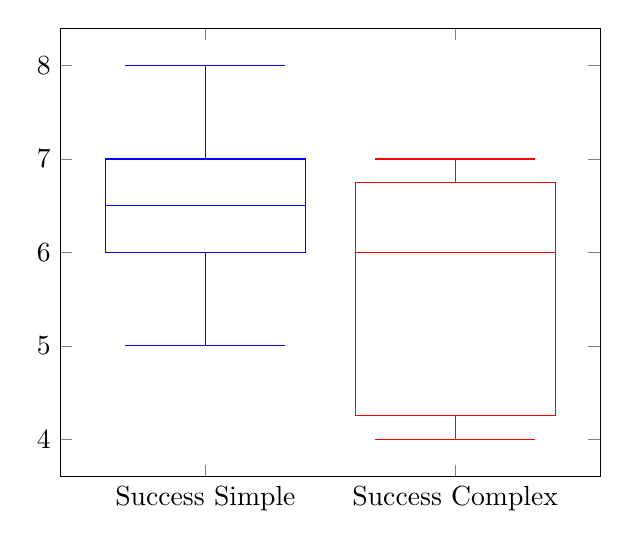
\begin{tikzpicture}
  \begin{axis}
    [
    boxplot/draw direction=y,
    xtick={1,2},
    xticklabels={Success Simple, Success Complex},
    ]
    \addplot+[
    boxplot prepared={
      median=6.5,
      upper quartile=7,
      lower quartile=6,
      upper whisker=8,
      lower whisker=5
    },
    ] coordinates {};
    \addplot+[
    boxplot prepared={
      median=6,
      upper quartile=6.75,
      lower quartile=4.25,
      upper whisker=7,
      lower whisker=4
    },
    ] coordinates {};
  \end{axis}
\end{tikzpicture}
    \caption{The results of Hypothesis 2 testing represented in a Box Plot}
    \label{fig:boxPlotHyp2}
\end{figure}

The results for the t test for this hypothesis returned a p value of 0.011449747 which is less than 0.05 which means the null hypothesis can be rejected. Therefore H1 is accepted which states that	there	is a significant difference in	the	detection (access)	rate	between	a	simple	and	a	complex	pattern	of	a password.

\subsection{Hypothesis 3}
\begin{center}
\textit{The	effect	from	adding	the	ID	rhythm. That there is an effect from the ID entry rhythm which has an affect on the detection rate.} \newline \\

\textbf{H0:} \textit{That adding the ID	into the pattern makes no significant difference in the detection rate.} \newline \\
\textbf{H1:} \textit{That adding the ID	into the pattern makes a significant	difference in the detection	rate.} \newline \\
\end{center}

For this hypothesis I repeated the experiment of hypothesis 2, however I included the username in the rhythm creator. This would mean that the user's typing characteristics for both the entrance of their username and password were recorded by the system and added to a profile.  

{
\begin{table} [H]
\centering
\begin{tabular}{ |p{2cm}|p{4cm}|p{4cm}| p{4cm} | }
\hline
\multicolumn{4}{|c|}{\textbf{Hypothesis 3 Testing Results (Simple Rhythm)}} \\
\hline
\textbf{Participant} & \textbf{Success without Username} & \textbf{Success with Username} & \textbf{Total Success Percentage} \\
\hline
1 & 7 & 6 & 65\% \\
\hline
2 & 8 & 8 & 80\% \\
\hline
3 & 7 & 5 & 60\% \\
\hline
4 & 6 & 5 & 55\%  \\
\hline
5 & 6 & 4 & 50\% \\
\hline
6 & 5 & 3 & 40\% \\
\hline
7 & 8 & 6 & 70\% \\
\hline
8 & 6 & 4 & 50\% \\
\hline
9 & 7 & 7 & 70\% \\
\hline
10 & 7 & 6 & 65\% \\
\hline
\textbf{Total} & \textbf{66} & \textbf{54} & \\
\hline
\textbf{Average} & \textbf{6.7} & \textbf{5.4} & \textbf{60.5\%} \\
\hline
\textbf{Maximum} & \textbf{8} & \textbf{8} & \textbf{80\%} \\
\hline
\textbf{Minimum} & \textbf{5} & \textbf{3} & \textbf{40\%} \\
\hline
\textbf{Range} & \textbf{3} & \textbf{5} & \textbf{40\%} \\
\hline
\textbf{Median} & \textbf{7} & \textbf{5.5} & \\
\hline
\textbf{Lower Quartile} & \textbf{6} & \textbf{4.25} & \\
\hline
\textbf{Upper Quartile} & \textbf{7} & \textbf{6} & \\
\hline
\end{tabular}
\caption{Table shows results of testing for Hypothesis 3 with the simple rhythm credentials}
\label{table:3}
\end{table}
}

Table \ref{table:3} shows that the total number of successes using a simple rhythm password without a username was 66 this figure decreased to 54 when a username was introduced. Along with this the average number of successes was 6.7 without a username and again this fell to 5.4 when a username was introduced. The median value further demonstrates this downward trend as it is 7 for a simple rhythm password without a username and the median value when a username was introduced was 5.5.  \\

The results for the t test for this hypothesis returned a p value of 0.000372809 which is less than 0.05 which means the null hypothesis can be rejected. Therefore H1 is accepted which states that adding the ID into the pattern makes a significant	difference in the detection	rate for simple passwords, for this to hold globally H1 must also be accepted for complex rhythms. 

{
\begin{table} [H]
\centering
% TODO Table: First 5 participants simple rythm password
\begin{tabular}{ |p{2cm}|p{4cm}|p{4cm}| p{4cm} | }
\hline
\multicolumn{4}{|c|}{\textbf{Hypothesis 3 Testing Results (Complex Rhythm)}} \\
\hline
\textbf{Participant} & \textbf{Success without Username} & \textbf{Success with Username} & \textbf{Total Success Percentage} \\
\hline
1 & 6 & 5 & 55\% \\
\hline
2 & 7 & 4 & 55\% \\
\hline
3 & 7 & 5 & 60\% \\
\hline
4 & 6 & 3 & 45\%  \\
\hline
5 & 5 & 4 & 45\% \\
\hline
6 & 5 & 3 & 40\% \\
\hline
7 & 6 & 6 & 60\% \\
\hline
8 & 4 & 3 & 35\% \\
\hline
9 & 7 & 5 & 60\% \\
\hline
10 & 5 & 3 & 40\% \\
\hline
\textbf{Total} & \textbf{58} & \textbf{41} & \\
\hline
\textbf{Average} & \textbf{5.8} & \textbf{4.1} & \textbf{49.5\%} \\
\hline
\textbf{Maximum} & \textbf{7} & \textbf{6} & \textbf{60\%} \\
\hline
\textbf{Minimum} & \textbf{4} & \textbf{3} & \textbf{35\%} \\
\hline
\textbf{Range} & \textbf{3} & \textbf{3} & \textbf{25\%} \\
\hline
\textbf{Median} & \textbf{6} & \textbf{4} & \\
\hline
\textbf{Lower Quartile} & \textbf{5} & \textbf{3} & \\
\hline
\textbf{Upper Quartile} & \textbf{6.75} & \textbf{5} & \\
\hline
\end{tabular}
\caption{Table shows results of testing for Hypothesis 3 with the complex rhythm credentials}
\label{table:4}
\end{table}
}

Table \ref{table:4} shows that the total number of successes using a complex rhythm password without a username was 58 this figure decreased to 41 when a username was introduced. Furthermore, the average number of successes was 5.8 without a username and again this fell to 4.1 when a username was introduced to the experiment. The median value of the complex rhythm without a username was 6 and this again fell to 4 when a username wad added. \\

The t test results for complex passwords returned a p value of 0.000153511 which is less than 0.05 which shows the difference between entering a complex password only and complex username and password entry is statistically significant which means the null hypothesis can be rejected. Therefore H1 is accepted which states that adding the ID into the pattern makes a significant difference in the detection rate for complex passwords. This means that hypothesis held in both cases involving simple and complex passwords. Thus, the conclusion could be made that the introduction of a username affects the success of a keystroke dynamic system.  \\

The results from both Table \ref{table:3} and Table \ref{table:4} are represented in Figure \ref{fig:boxPlotHyp3}. This illustrates the general trend that when a username is introduced the number of successful attempts decreases. As both points SNU and CNU are much higher than SU and CU. In addition, there is no overlap between each of the pairs of values.   

\begin{figure} [H]
    \centering
    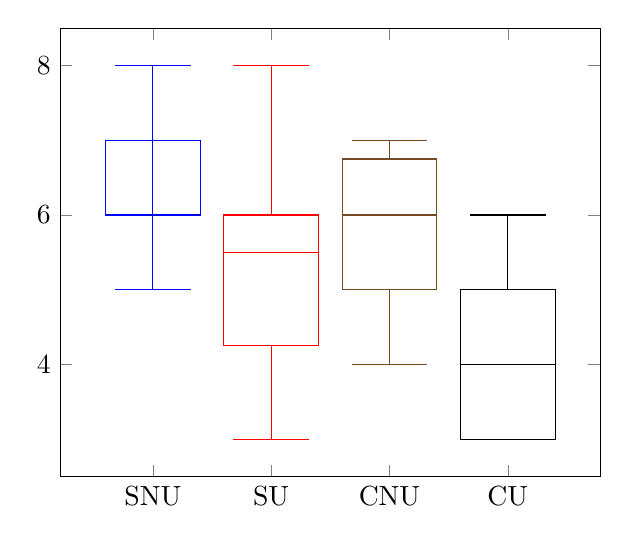
\begin{tikzpicture}
  \begin{axis}
    [
    boxplot/draw direction=y,
    xtick={1,2,3,4},
    xticklabels={SNU, SU, CNU, CU},
    ]
    \addplot+[
    boxplot prepared={
      median=7,
      upper quartile=6,
      lower quartile=7,
      upper whisker=8,
      lower whisker=5
    },
    ] coordinates {};
    \addplot+[
    boxplot prepared={
      median=5.5,
      upper quartile=6,
      lower quartile=4.25,
      upper whisker=8,
      lower whisker=3
    },
    ] coordinates {};
    \addplot+[
    boxplot prepared={
      median=6,
      upper quartile=6.75,
      lower quartile=5,
      upper whisker=7,
      lower whisker=4
    },
    ] coordinates {};
    \addplot+[
    boxplot prepared={
      median=4,
      upper quartile=5,
      lower quartile=3,
      upper whisker=6,
      lower whisker=3
    },
    ] coordinates {};
  \end{axis}
\end{tikzpicture}
    \caption{The results of Hypothesis 3 testing represented in a Box Plot. Key: Simple No Username (SNU), Simple Username (SU), Complex No Username (CNU), Complex Username}
    \label{fig:boxPlotHyp3}
\end{figure}

\subsection{Hypothesis 4} \label{hypo4}
\begin{center}
\textit{That there is a length L over which the timings of the password and ID are
irrelevant. That is, L is more predictive of detection than rhythm when L $\geq$ N characters.} \newline \\

\textbf{H0:} \textit{There	is	no	length	L	(=ID+PW) which	effects	a	change	in	the	rhythm detection	rate.} \newline \\

\textbf{H1:} \textit{There	is	a	length	L	which	affects	the	rhythm	detection	rate.}
\end{center}

For this hypothesis I created three sets of username and password combinations, short (12 characters), medium (20 characters) and long (36 characters). These pairs are shown in the list below: 

\begin{enumerate}
    \item Small - ID: abcdef, Password: asdfgh
    \item Medium - ID: abcdef1056, Password: asdfghjk10
    \item Long - ID:abcdef10567, Password: asdfghjk10lmnbv
\end{enumerate}

{
\begin{table} [H]
\centering
\begin{tabular}{ |p{2cm}|p{2cm}|p{2cm}| p{2cm}| p{2cm}| }
\hline
\multicolumn{5}{|c|}{\textbf{Hypothesis 4 Testing Results}} \\
\hline
\textbf{Participant} & \textbf{Success short} & \textbf{Success medium} & \textbf{Success long}  & \textbf{Total Success Percentage} \\
\hline
1 & 8 & 6 & 5 & 63.33\% \\
\hline
2 & 7 & 7 & 6 & 66.66\% \\
\hline
3 & 7 & 4 & 4 & 50\% \\
\hline
4 & 9 & 7 & 6 & 73.33\%  \\
\hline
5 & 8 & 5 & 4 & 56.66\% \\
\hline
6 & 5 & 2 & 1 & 26.66\% \\
\hline
7 & 7 & 6 & 4 & 56.66\% \\
\hline
8 & 6 & 4 & 3 & 43.33\% \\
\hline
9 & 7 & 5 & 4 & 53.33\% \\
\hline
10 & 6 & 4 & 2 & 40\% \\
\hline
\textbf{Total} & \textbf{70} & \textbf{50} & \textbf{39} & \\
\hline
\textbf{Average} & \textbf{7} & \textbf{5} & \textbf{3.9} & \textbf{53\%} \\
\hline
\textbf{Maximum} & \textbf{9} & \textbf{7} & \textbf{6} & \textbf{80\%} \\
\hline
\textbf{Minimum} & \textbf{5} & \textbf{2} & \textbf{1} & \textbf{26.66\%} \\
\hline
\textbf{Range} & \textbf{4} & \textbf{5} & \textbf{5} & \textbf{46.66\%} \\
\hline
\textbf{Median} & \textbf{7} & \textbf{5} & \textbf{4} & \\
\hline
\textbf{Lower Quartile} & \textbf{6.25} & \textbf{4} & \textbf{3.25} &  \\
\hline
\textbf{Upper Quartile}& \textbf{7.75} & \textbf{6} & \textbf{4.75} &  \\
\hline
\end{tabular}
\caption{Table shows results of testing for Hypothesis 4 with the differing length of credentials}
\label{table:5}
\end{table}
}

Table \ref{table:5} illustrates the results of the Hypothesis 4 experiment. It shows a clear downward trend in the number of successes as the length of the string increases. As the total number of successes for a short length password is 70 this falls to 50 when the password length was increased to the medium length and the number of successes drops to 39 for long password strings. This downward trend is also shown in Figure \ref{fig:boxPlotHyp4}. 

\begin{figure} [H]
    \centering
    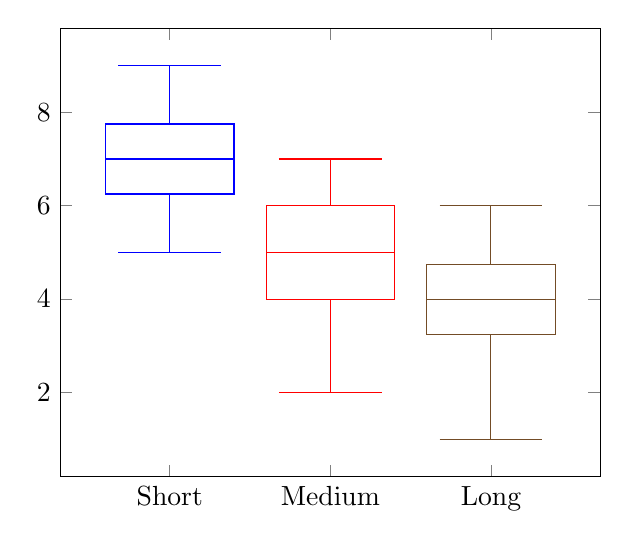
\begin{tikzpicture}
  \begin{axis}
    [
    boxplot/draw direction=y,
    xtick={1,2,3},
    xticklabels={Short, Medium, Long},
    ]
    \addplot+[
    boxplot prepared={
      median=7,
      upper quartile=7.75,
      lower quartile=6.25,
      upper whisker=9,
      lower whisker=5
    },
    ] coordinates {};
    \addplot+[
    boxplot prepared={
      median=5,
      upper quartile=6,
      lower quartile=4,
      upper whisker=7,
      lower whisker=2
    },
    ] coordinates {};
     \addplot+[
    boxplot prepared={
      median=4,
      upper quartile=4.75,
      lower quartile=3.25,
      upper whisker=6,
      lower whisker=1
    },
    ] coordinates {};
  \end{axis}
\end{tikzpicture}
    \caption{The results of Hypothesis 4 testing}
    \label{fig:boxPlotHyp4}
\end{figure}

In accordance with the specification the difference is statistically significant if: 
\begin{center}
    $ |IDPW.numlt12(success)| < |IDPW.numlt12(success) \times 1.1| $ AND \\
    $ |IDPW.numgt12(success)| < |IDPW.numlt20(success) \times 1.1| $ AND \\
    $ |IDPW.numgt12(success)| < |IDPW.numlt36(success) \times 1.1| $ \\
\end{center} 

\begin{center}
    $ |70| < |77| $ AND \\
    $ |70| < |55| $ AND \\
    $ |70| < |42.9| $ \\
\end{center} 


The results of this experiment prove H1 that there	is	a length L	which	affects	the	rhythm	detection	rate. As the second and third comparisons in the equation do not evaluate to true, as 70 is greater than both 55 and 42.9. This could be an area for future research to identify exactly at what length of string the success of the rhythm authentication becomes less viable, I would propose however it is in the range of 20-30 characters. 


\subsection{Extension: Hypothesis 5}
\begin{center}
\textit{Does the meaning of a word within a password have any effect on the success of a user logging in? Comparing a password with meaning versus a password without meaning} \newline \\
\textbf{H0:} \textit{The meaning of a word has no effect on the successful entry rate} \newline \\
\textbf{H1:} \textit{The meaning of a word has an effect on the successful entry rate}
\end{center}

For this experiment I assigned users with a password with a meaningful word involved, banana6789 and contrasted this with a password with no meaning, yuvb10q5a9.  

{
\begin{table} [H]
\centering
% TODO Table: First 5 participants simple rythm password
\begin{tabular}{ |p{2cm}|p{4cm}|p{4cm}| p{4cm} | }
\hline
\multicolumn{4}{|c|}{\textbf{Hypothesis 5 Testing Results}} \\
\hline
\textbf{Participant} & \textbf{Success Meaning} & \textbf{Success no Meaning} & \textbf{Total Success Percentage} \\
\hline
1 & 8 & 7 & 75\% \\
\hline
2 & 7 & 7 & 70\% \\
\hline
3 & 7 & 6 & 65\% \\
\hline
4 & 9 & 8 & 85\%  \\
\hline
5 & 8 & 8 & 80\% \\
\hline
6 & 7 & 6 & 65\% \\
\hline
7 & 7 & 7 & 70\% \\
\hline
8 & 6 & 6 & 60\% \\
\hline
9 & 7 & 6 & 65\% \\
\hline
10 & 8 & 7 & 75\% \\
\hline
\textbf{Total} & \textbf{74} & \textbf{68} & \\
\hline
\textbf{Average} & \textbf{7.4} & \textbf{6.8} & \textbf{71\%} \\
\hline
\textbf{Maximum} & \textbf{9} & \textbf{8} & \textbf{85\%} \\
\hline
\textbf{Minimum} & \textbf{6} & \textbf{6} & \textbf{60\%} \\
\hline
\textbf{Range} & \textbf{3} & \textbf{2} & \textbf{25\%} \\
\hline
\textbf{Median} & \textbf{7} & \textbf{7} & \\
\hline
\textbf{Lower Quartile} & \textbf{7} & \textbf{6} & \\
\hline
\textbf{Upper Quartile} & \textbf{8} & \textbf{7} & \\
\hline
\end{tabular}
\caption{Table shows results of testing for Hypothesis 5 with the complex rhythm credentials}
\label{table:6}
\end{table}
}

Table \ref{table:6} shows the results of contrasting the meaningful password with a password with no meaning. The results show that users logged in more successfully when using the password that had meaning. A rationale for this result could be it requires much less memory to type a word they know than to memorise a non descriptive 10 letter password. The results are graphically displayed in Figure \ref{fig:boxPlotHyp5}, there is little overlap between the two boxes, although both entrance criteria were largely successful the attempts using a word with meaning were more successful than using a string without meaning. However, this must be repeated with a variety of different passwords and a much wider participant base for the results to be considered substantial. 

\begin{figure} [H]
    \centering
    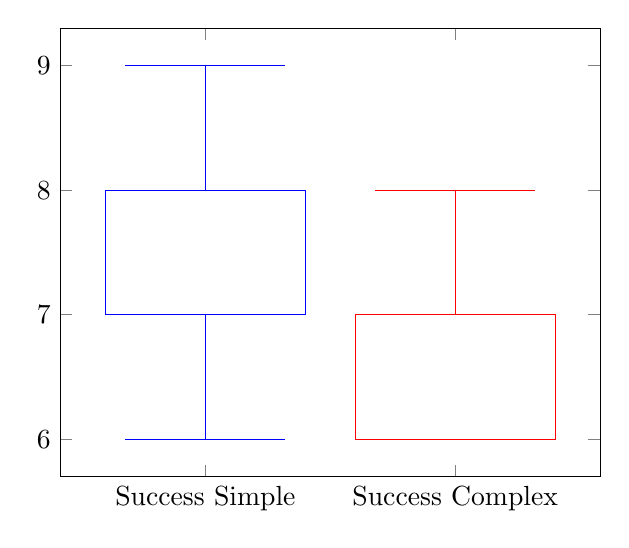
\begin{tikzpicture}
  \begin{axis}
    [
    boxplot/draw direction=y,
    xtick={1,2},
    xticklabels={Success Simple, Success Complex},
    ]
    \addplot+[
    boxplot prepared={
      median=7,
      upper quartile=8,
      lower quartile=7,
      upper whisker=9,
      lower whisker=6
    },
    ] coordinates {};
    \addplot+[
    boxplot prepared={
      median=7,
      upper quartile=7,
      lower quartile=6,
      upper whisker=8,
      lower whisker=6
    },
    ] coordinates {};
  \end{axis}
\end{tikzpicture}
    \caption{The results of Hypothesis 5 testing}
    \label{fig:boxPlotHyp5}
\end{figure}

The t test value returned for this hypothesis was 0.002560536 which is less than 0.05 therefore the difference between the two result sets is statistically significant. Therefore the null hypothesis can be rejected and H1 can be accepted. These results imply that users are more successful entering a password when it is a meaningful into a keystroke dynamics monitoring system. This hypothesis would be an interesting area to focus on in future research, as it could have far reaching consequences for the development of keystroke dynamics systems.  

\subsection{Extension: Hypothesis 6}
\begin{center}
\textit{Does the complexity of the memory tasks involved with passwords have an effect on success rate of passwords?} \newline \\
\textbf{H0:} \textit{The complexity of memorising the password has no effect on the successful entry rate} \newline \\
\textbf{H1:} \textit{The complexity of memorising the password has an effect on the successful entry rate}
\end{center}

For this hypothesis I tested the password entry of users using a simple to memorise password and a complex to memorise password. Simple password: asdfghjk and Complex password: wdxcybza. 


{
\begin{table} [H]
\centering
% TODO Table: First 5 participants simple rythm password
\begin{tabular}{ |p{2cm}|p{4cm}|p{4cm}| p{4cm} | }
\hline
\multicolumn{4}{|c|}{\textbf{Hypothesis 6 Testing Results}} \\
\hline
\textbf{Participant} & \textbf{Success Simple Memory} & \textbf{Success Complex Memory} & \textbf{Total Success Percentage} \\
\hline
1 & 8 & 5 & 65\% \\
\hline
2 & 7 & 5 & 60\% \\
\hline
3 & 8 & 5 & 65\% \\
\hline
4 & 9 & 6 & 75\%  \\
\hline
5 & 8 & 6 & 70\% \\
\hline
6 & 6 & 3 & 45\% \\
\hline
7 & 7 & 5 & 60\% \\
\hline
8 & 6 & 4 & 50\% \\
\hline
9 & 7 & 3 & 50\% \\
\hline
10 & 7 & 6 & 65\% \\
\hline
\textbf{Total} & \textbf{73} & \textbf{48} & \\
\hline
\textbf{Average} & \textbf{7.3} & \textbf{4.8} & \textbf{60.5\%} \\
\hline
\textbf{Maximum} & \textbf{9} & \textbf{6} & \textbf{75\%} \\
\hline
\textbf{Minimum} & \textbf{6} & \textbf{3} & \textbf{45\%} \\
\hline
\textbf{Range} & \textbf{3} & \textbf{3} & \textbf{30\%} \\
\hline
\textbf{Median} & \textbf{7} & \textbf{5} & \\
\hline
\textbf{Lower Quartile} & \textbf{7} & \textbf{4.25} & \\
\hline
\textbf{Upper Quartile} & \textbf{8} & \textbf{5.75} & \\
\hline
\end{tabular}
\caption{Table shows results of testing for Hypothesis 6}
\label{table:7}
\end{table}
}

Table \ref{table:7} shows the results of the hypothesis 6 experiment. Largely it showed that users were more successful at logging in when the password supplied was a simple memory task in comparison to a complex memory task. The total number of successes with a simple password was 73 this dramatically fell to 48 for a complex memory password. Along with this the average of the two results set show that simple memory passwords had an average of 7.3 successful entries which dropped to 4.8 when the complex memory password was introduced. Figure \ref{fig:boxPlotHyp6} shows the difference between the two result sets such that the simple memory results largely sit at the top end of the results spectrum and the complex memory password results are significantly lower. 

\begin{figure} [H]
    \centering
    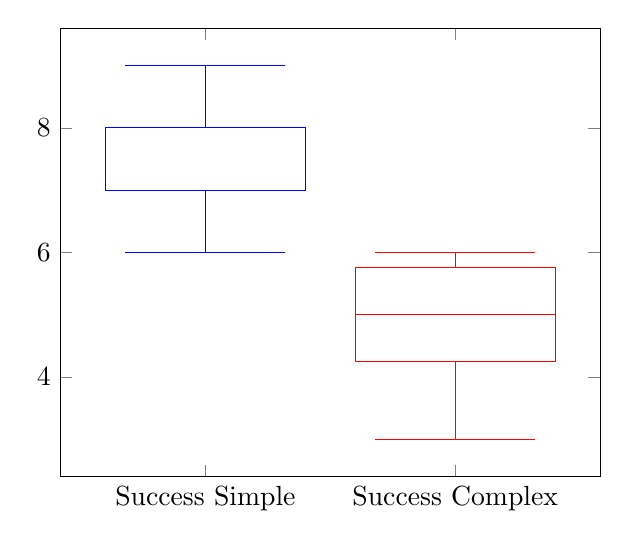
\begin{tikzpicture}
  \begin{axis}
    [
    boxplot/draw direction=y,
    xtick={1,2},
    xticklabels={Success Simple, Success Complex},
    ]
    \addplot+[
    boxplot prepared={
      median=7,
      upper quartile=8,
      lower quartile=7,
      upper whisker=9,
      lower whisker=6
    },
    ] coordinates {};
    \addplot+[
    boxplot prepared={
      median=5,
      upper quartile=5.75,
      lower quartile=4.25,
      upper whisker=6,
      lower whisker=3
    },
    ] coordinates {};
  \end{axis}
\end{tikzpicture}
    \caption{The results of Hypothesis 6 testing represented in a Box Plot}
    \label{fig:boxPlotHyp6}
\end{figure}

The t test value returned for this hypothesis was 0.000003255 which is significantly less than 0.05 therefore the difference between the two result sets is statistically significant. Therefore the null hypothesis can be rejected and H1 can be accepted. These results affirm the intuitive hypothesis that a complex memory password is harder to enter into a keystroke dynamics system than a password which is much less taxing to memorise. This would imply that users may make mistakes or be infrequent in timing when typing due to how hard they find it memorise a password.

\section{Difficulties}
Having never conducted experimental research utilising statistics before I found this practical challenging as once I had implemented the program and collected the results I feel I spent a disproportional amount of time learning how to analyse this data. Although the analysis is good I do feel prior experience with statistics would have given me a more sound base to begin with which may have improved this section of the practical. Overall, I found this practical extremely interesting and this why I spent such a large amount of time on it as it was something which I think could be viable for implementation in authentication systems. In the future I would be very interested to keep up to date with research in this field and potentially conduct my own further research. 

\section{Future Work} \label{futureWork}
For this experiment to have real scientific weight it would need to be completed at a much larger scale with an increased number of participants from a variety of demographics. It would be very interesting to test the viability of typing characteristics in an authentication environment as it could enhance the security of a large range of systems that are reliant upon traditional username and password authentication. One area which requires a depth of future research is the threshold at which a timing value is accepted as if this value is too little it may make logging in for legitimate users more complicated which in turn would be detrimental to the uptake of the typing characteristics in an authentication environment. Conversely, if this value is too lenient it may allow illegitimate users access to a system which make it no more secure than the traditional username and password authentication. This threshold value would be crucial to the adoption of keystroke dynamics.  \\

Furthermore, it would be interesting to inspect the performance of keystroke dynamic systems in tandem with human factors such as tiredness (as I imagine users would type differently depending upon the time of day), different physical and language keyboards. These areas would provide further insight into the possibility of these keystroke dynamics systems becoming ubiquitous.   

\section{Conclusion}
% My experiment summary
This experiment has provided some results based on an implementation of a rhythmic keylogger for authentication. It has shown that users are less successful at logging in when passwords are distributed around the keyboard, when passwords contain complex patterns, that the introduction of username entry negatively affects the success rate of user authentication and that as credentials get longer the success rate of users authentication worsens. Along with this I tested two of my own hypothesis that users will be more successful at logging in when using words with meaning and that the more complex the memory task involved in password entry the smaller the success rate will be, both of which were shown to be true via experimentation. There is large scope for further research in this area as discussed in Section \ref{futureWork} even repeating this experiment with a much larger and demographically distributed users would produce valuable results.  \\

% General KD
In general there is a large chance of the widespread adoption of keystroke dynamics as it does not compromise usability for the purpose of security and the process is transparent to the user. In the future, the techniques used in keystroke dynamics are likely to become extremely high entropy as algorithms and the resources of computer systems improve at a formidable rate, this will subsequently improve all forms of authentication security as keystroke dynamics in tandem with login credentials becomes the secure standard. This is a field that blends the lines between computer security and biometrics, which makes it of high interest in the research industry but the approach also has many practical applications. Personally, I hope that systems adopt this approach as it may make authentication a much more secure process.  

\section{Appendix: Code Listings} \label{appendix}

\subsection{Profile Creation}
The following methods were utilised to record the time a user pressed a key for as well as the time between keypresses. These methods utilise the Apache Commons StopWatch( \url{http://bit.ly/2275sOL}) class to record the timings.  

\begin{lstlisting}
    /**
     * Handle the key pressed event from the text field.
     */

    @Override
    public void keyPressed(KeyEvent e) {
        int textFieldEntered = 0;

        if (e.getSource() == txtUser) {
            System.out.println("Key pressed in txtUser1");
            textFieldEntered = 1;
            recordTimeBetweenKeys(textFieldEntered);
        }
        if (e.getSource() == pass) {
            System.out.println("Key pressed in pass");
            textFieldEntered = 2;
            recordTimeBetweenKeys(textFieldEntered);
        }
    }

    /**
     * Handle the key released event from the text field.
     */

    @Override
    public void keyReleased(KeyEvent e) {
        int textFieldEntered = 0;
        if (e.getSource() == txtUser) {
            System.out.println("Key released in txtUser1");
            textFieldEntered = 1;
        }
        if (e.getSource() == pass) {
            System.out.println("Key released in pass");
            textFieldEntered = 2;
        }
        recordTime(textFieldEntered);
    }

    private void recordTimeBetweenKeys(int textFieldEntered) {
        if (textFieldEntered == 0) {
            System.out.println("recordTimeBetweenKeys textFieldEntered was 0 error");
            System.exit(1);
        }
        if (textFieldEntered == 1) {
            if (usernameTimings.size() == 0) {
                stopWatchUsername.start();
            } else {
                long time = stopWatchUsername.getTime();
                System.out.println("time between key is: " + time);
                usernameTimings.add(time);
                stopWatchUsername.reset();
                stopWatchUsername.start();
            }
        } else if (textFieldEntered == 2) {
            if (passwordTimings.size() == 0) {
                stopWatchPassword.start();
            } else {
                long time = stopWatchPassword.getTime();
                System.out.println("time between key is: " + time);
                passwordTimings.add(time);
                stopWatchPassword.reset();
                stopWatchPassword.start();
            }
        }
    }


    /**
     * Records the time to the users profile.
     */
    private void recordTime(int textFieldEntered) {
        if (textFieldEntered == 0) {
            System.out.println("textFieldEntered was 0 error");
            System.exit(1);
        }
        if (textFieldEntered == 1) {
            stopWatchUsername.stop();
            long time = stopWatchUsername.getTime();
            System.out.println("text 1 key held time is : " + time);
            usernameTimings.add(time);
            stopWatchUsername.reset();
            stopWatchUsername.start();
        } else if (textFieldEntered == 2) {
            stopWatchPassword.stop();
            long time = stopWatchPassword.getTime();
            System.out.println("pass key held time is : " + time);
            passwordTimings.add(time);
            stopWatchPassword.reset();
            stopWatchPassword.start();
        }
    }
\end{lstlisting}

\subsection{Rhythm checker}
This code is utilised when registering a user to ensure that the values of each of the timings arrays are within the threshold value (which is set globally at 100ms) of one another.I chose to use array lists for timings with the values added being the the time a key was pressed for (key released - key pressed) and the time between key presses.
\begin{lstlisting}
    public boolean entriesWithinThresholdUsername() {
        boolean match = false;
        for (int i = 0; i < username1Timings.size(); ) {
            for (int j = 0; j < username2Timings.size(); j++) {
                long val = Math.abs(username1Timings.get(i).longValue()
                        - username2Timings.get(j).longValue());
                if (val <= threshold) {
                    match = true;
                    i++;
                } else {
                    return false;
                }
            }
        }
        return match;
    }

    private boolean entriesWithinThresholdPassword() {
        boolean match = false;
        for (int i = 0; i < password1Timings.size(); ) {
            for (int j = 0; j < password2Timings.size(); j++) {
                if (Math.abs(password1Timings.get(i).longValue()
                        - password2Timings.get(j).longValue()) <= threshold) {
                    match = true;
                    i++;
                } else {
                    return false;
                }
            }
        }
        return match;
    }
\end{lstlisting}

\subsection{Persistent Storage of User Profiles}
I utilised the Java Serilizable API to write user profiles to a persistent file for storage. 
\begin{lstlisting}
    public void seralizeUser() {
        String passwordToHash = user.getPassword();
        String securePassword = get_SHA_256_SecurePassword(passwordToHash);
        user.setPassword(securePassword);
        try {
            FileOutputStream fileOut =
                    new FileOutputStream("./Storage/users.ser", true);
            ObjectOutputStream out = new ObjectOutputStream(fileOut);
            out.writeObject(user);
            out.flush();
            out.close();
            fileOut.flush();
            fileOut.close();
        } catch (IOException i) {
            i.printStackTrace();
        }
    }

    public ArrayList<User> deseralizeUser() {
        ArrayList<User> savedUsers = new ArrayList<>();
        try {
            FileInputStream fileIn = new FileInputStream("./Storage/users.ser");
            while (true) {
                ObjectInputStream in = new ObjectInputStream(fileIn);
                try {
                    User u = (User) in.readObject();
                    savedUsers.add(u);
                } catch (EOFException e) {
                    // Close readers
                    in.close();
                    fileIn.close();
                    return savedUsers;
                }
            }
        } catch (IOException i) {
            i.printStackTrace();
        } catch (ClassNotFoundException c) {
            System.out.println("User class not found");
            c.printStackTrace();
        }
        return savedUsers;
    }
\end{lstlisting}

\subsection{Password Hashing}
I used a SHA-256 Hash to store the passwords of users to ensure that they were stored safely. 

\begin{lstlisting}
    public String get_SHA_256_SecurePassword(String passwordToHash) {
        String generatedPassword = null;
        try {
            MessageDigest md = MessageDigest.getInstance("SHA-256");
            byte[] bytes = md.digest(passwordToHash.getBytes());
            StringBuilder sb = new StringBuilder();
            for (int i = 0; i < bytes.length; i++) {
                sb.append(Integer.toString((bytes[i] & 0xff) + 0x100, 16).substring(1));
            }
            generatedPassword = sb.toString();
        } catch (NoSuchAlgorithmException e) {
            e.printStackTrace();
        }
        return generatedPassword;
    }
\end{lstlisting}

\medskip
\printbibliography


\end{document}
